
%(BEGIN_QUESTION)
% Copyright 2010, Tony R. Kuphaldt, released under the Creative Commons Attribution License (v 1.0)
% This means you may do almost anything with this work of mine, so long as you give me proper credit

Suppose we have an Allen-Bradley model ``SLC 500'' PLC connected to three pushbutton switches and two lamps as shown in this illustration:

$$\includegraphics[width=15.5cm]{i04671x01.eps}$$

Examine the following relay ladder logic (RLL) program for this Allen-Bradley PLC, determining the statuses of the two lamps provided switches A and B are pressed, and switch C is unpressed:

$$\includegraphics[width=15.5cm]{i04671x02.eps}$$

\underbar{file i04671}
%(END_QUESTION)





%(BEGIN_ANSWER)

Lamp Y is de-energized.

\vskip 10pt

Lamp Z is de-energized.

%(END_ANSWER)





%(BEGIN_NOTES)

{\bf This question is intended for exams only and not worksheets!}.

%(END_NOTES)


